\subsection{fulibWorkflows}\label{subsec:fulibworkflows}
Bei~\textit{fulibWorkflows} handelt es sich um eine Java-Bibliothek, welche Workflows in YAML\footnote{Kurzform von ``YAML Ain't Markup Language''}-Syntax notiert,
als Eingabe erhält und daraus
sowohl ein \ac{ES}-Board als auch im Workflow beschriebene Mockups und Objekt-/ Klassendiagramme generiert.
Welche Form die YAML-Eingabe haben muss und wie die Dateien aussehen und generiert werden, wird in Kapitel~\ref{subsec:workflow-format} erläutert.

\subsubsection{Antlr}\label{subsubsec:antlr}
\ac{Antlr} bietet die Möglichkeit einen Parser über eine eigens geschriebene Grammatik zu generieren.
Die Grammatik muss linksableitend sein und ist in erweiterter Backus-Naur-Form definiert.
Der generierte Parser ermöglicht zudem das Aufbauen und Ablaufen eines~\textit{Parse trees}.
Bei einem~\textit{Parse tree} handelt es sich um einen Syntaxbaum, in welchem über eine hierarchische Struktur ein Text in mehrere Knoten unterteilt wird.
Hierdurch ergibt sich die Möglichkeit, während dem Parsen weitere Aktionen durchzuführen, welche den späteren Programmablauf eines Tools unterstützen können.

\begin{listing}[!ht]
    \inputminted{antlr-java}{listings/2.2.1/AntlrExample.g4}
    \caption{Beispiel einer einfachen Grammatik in Antlr}
    \label{listing:grammar-example}
\end{listing}

In Listing~\ref{listing:grammar-example} ist ein Beispiel für eine einfache Grammatik zur Erkennung von Wertzuweisungen beziehungsweise dem Erstellen von
Properties dargestellt.\cite*{antlrOrg}
Es existieren drei nicht-terminale Regeln, welche für den generierten Parser wichtig sind, und den Gesamtaufbau einer Eingabe definieren.
Die Grammatik kann mehrere Properties verarbeiten, welche aus einer ID, einem Gleichheitszeichen und einem Wert bestehen.
Hierbei ist in Zeile 4 zu erkennen, dass nach jeder Property eine neue Zeile begonnen werden muss.
Ein Wert kann entweder ein String oder eine ID sein.
\textit{STRING} und \textit{ID} sind terminale Regeln, welche einen finalen Knoten für einen Ast des Parse Trees darstellen.

Die zuvor beschriebene Grammatik kann mittels weiterer Tools auf eine Eingabe geprüft werden.
Eine zulässige Eingabe für die festgelegte Grammatik aus Listing~\ref{listing:grammar-example} ist in Listing~\ref{listing:prop-input} dargestellt.

\begin{listing}[!ht]
    \begin{minted}{text}
name=parrt
title="Supreme dictator for life"

    \end{minted}
    \caption{Eingabe}
    \label{listing:prop-input}
\end{listing}

Die Überprüfung auf die Richtigkeit einer Eingabe oder auch der Grammatik kann über Tools bereits vor einer Generierung von Code durchgeführt werden.
Hierzu wurde das Diagramm aus Abbildung~\ref{fig:parse-example} mittels des Antlr-Plugins für IntelliJ generiert.

\begin{figure}[h]
    \centering
    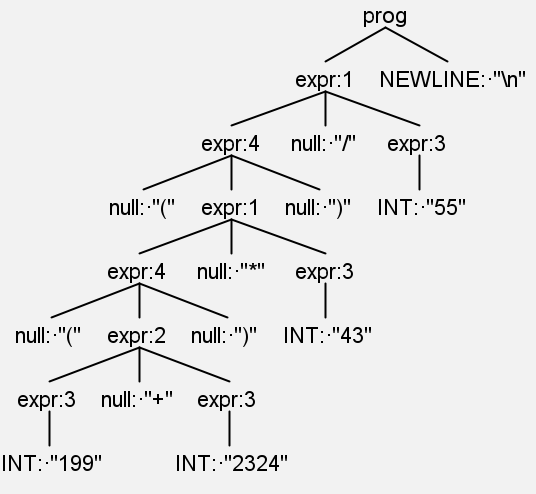
\includegraphics[width=0.5\textwidth]{images/2.2/parseTreeExample}
    \caption{Interner Parse Tree}
    \label{fig:parse-example}
\end{figure}

Hierbei ist ersichtlich, dass die Wurzel bei der obersten Regel~\textbf{file} beginnt und alle weiteren Kindknoten durch \textbf{prop} Regeln kreiert wurden.
Beide Properties besitzen eine ID und einen Wert, welcher durch ein Gleichheitszeichen und einen Zeilenumbruch umklammert ist.
Der zugeordnete Wert ist bei den Properties dieses Beispieles allerdings unterschiedlich in \textit{ID} und \textit{STRING} aufgeteilt.
Dies entsteht durch die Unterscheidung bei der Grammatik in Terminale und Nicht-Terminale.
Hierbei werden wie in Listing~\ref{listing:grammar-example} dargestellt nicht-terminale Regeln kleingeschrieben und terminale Regeln werden in Großbuchstaben verfasst.
In der vereinfachten Grammatik sind lediglich ganze Zahlen als Eingabe erlaubt.

Dies sind lediglich die Grundlagen von Antlr, auf die genauere Verwendung des generierten Parsers und Besonderheiten der Grammatik wird in Kapitel~\ref{subsec:antlr-grammatik},
anhand der Implementierung, eingegangen.

\subsubsection{StringTemplate}
Die Java-Bibliothek \textit{StringTemplate} gehört, wie das vorherige~\ac{Antlr}, zum~\textit{Antlr Project}.
\ac{Antlr} verwendet ebenfalls String-Templates zur Generierung von formatiertem Text, im Folgenden als \textit{Code} bezeichnet.
Templates (übersetzt: Schablonen) ermöglichen es zum Beispiel die feste Syntax einer Programmiersprache mit variablen Werten für
Variablen, Klassen und Methoden zu belegen.
Somit können die generellen Bausteine einer Sprache beliebig gefüllt werden.
Durch diese Funktionalität bieten sich \acp{ST} sehr gut zur Generierung von Dateien an.
Ursprünglich ist \textit{StringTemplate} eine Java-Bibliothek, jedoch wurden bereits Portierungen für C\#, Objective-C, JavaScript und Scala erstellt.

Die folgenden Erläuterungen beziehen sich jedoch auf die ursprüngliche Java-Version von~\textit{StringTemplate}, da diese in dieser Arbeit verwendet wird.
Die einfachste Möglichkeit für die Verwendung eines String Templates ist in Listing~\ref{listing:simpleTemplate} zu sehen.

\begin{listing}[!ht]
    \inputminted{java}{listings/2.2.1/JavaStringTemplateExample.java}
    \caption{``Hello World!'' - Beispiel mittels StringTemplate}
    \label{listing:simpleTemplate}
\end{listing}

Die Klasse \textit{ST} aus Zeile 3 kann mit einem String initialisiert werden.
In diesem Beispiel wurden als Begrenzer für das zu ersetzende Stück des Textes die Zeichen ``<''  und ``>'' verwendet.
Im Anschluss wird dem neuen \textit{ST}-Objekt mithilfe der add()-Methode ein bestimmter Wert hinzugefügt.
Der erste Parameter der Methode ist der Bezeichner innerhalb eines Templates, zu beachten ist die Angabe des Bezeichners ohne die Begrenzer.
Der Wert wird als zweiter Parameter übergeben und besitzt in diesem Beispiel den Text~\textbf{World}.
Um nun den fertig ersetzten Text aus dem Template und dem übergebenem Wert zu bekommen, muss auf dem \textit{ST}-Objekt die Methode render() aufgerufen werden.
Hierbei werden die Platzhalter des Templates durch den zuvor übergebenen Wert ersetzt und als String zurückgegeben.
In Zeile 6 wird nun abschließend der fertige Text ``Hello, World!''  auf der Konsole ausgegeben.
Dieses Beispiel entstammt der offiziellen Webseite von~\textit{StringTemplate}\cite*{stOrg}.

Für ein strukturiertes Arbeiten mit vielen Templates bietet \textit{StringTemplate} die Möglichkeit \acp{STG} zu erstellen.
Hierbei können mehrere Templates in einer Datei beschrieben werden, um aufeinander aufbauende Templates nicht im Code, sondern einer gesonderten Datei zu organisieren.
In diesen Dateien, welche die Dateiendung \textbf{.stg} tragen, können die Begrenzer (eng.: Delimiters) frei gewählt werden.
Dies ist je nach Kontext des Templates nötig, da zum Beispiel die Generierung von HTML-Dateien, welche ``<''  und ``>'' als Zeichen zum Abgrenzen von Bereichen verwenden,
mit den Standard-Begrenzern für einen Mehraufwand sorgt.
Bei der Wahl der Begrenzer sollte somit stets auf die Wahl der Zeichen im Kontext der zu generierenden Sprache geachtet werden.
Zum Parsen einer \ac{STG} wird ein mit Antlr generierter Parser verwendet\cite*{stgParser}.

\begin{listing}[ht]
    \inputminted{c}{listings/2.2.1/Example.stg}
    \caption{Beispiel einer .stg-Datei}
    \label{listing:stgFile}
\end{listing}

Wie zuvor beschrieben ist in Listing~\ref{listing:stgFile} zu erkennen, dass in Zeile 1 die Begrenzer auf ``\{'' und ``\}'' gesetzt wurden.
Dies hat den Hintergrund, dass in diesem Beispiel ein Text in eine HTML-Datei generiert werden soll.
Hierfür könnten auch die Standard-Begrenzer verwendet werden, allerdings müssten dann für Schlüsselwörter wie~\texttt{<span>} die Zeichen ``<'' und ``>'' mit einem führenden Backslash definiert werden.
Da dies für HTML-Dateien allerdings einen immensen Aufwand bedeutet, ist die Nutzung anderer Begrenzer sinnvoll.
In Zeile 3 werden für ein~\ac{ST} sowohl der Name des Templates als auch Übergabeparameter definiert.
Ein~\ac{ST} wird durch ``> >'' geschlossen.
Die Begrenzer in Zeile 5 zeigen, dass alles, was sich zwischen Ihnen befindet, einen Übergabeparameter in sich trägt.
Somit ist das Wiederverwenden des Templates und die variable Befüllung gewährleistet.

Um diese Templates nun in einem Java-Programm zu verwenden, benötigt es unter anderem die zuvor beschriebene ST-Klasse, sowie
die Klasse~\textit{STGroupFile}, welche für die Verwaltung der stg-Datei als auch deren Templates, benötigt wird.
In Zeile 6 von Listing~\ref{listing:stgJavaFile} ist zu erkennen, dass einem STGroupFile-Objekt bei der Initialisierung eine URL übergeben werden muss.
Diese URL verweist auf die stg-Datei.
Im Anschluss kann, wie in Zeile 8 ersichtlich, über die getInstanceOf()-Methode auf ein bestimmtes Template in der stg-Datei zugegriffen werden.
Hierbei ist es wichtig, dass der übergebene Bezeichner der getInstanceOf()-Methode mit dem Bezeichner in der stg-Datei übereinstimmt.
Schließlich ist die weiterführende Verwendung bereits zuvor mittels der ST-Klasse beschrieben worden.

\begin{listing}[!ht]
    \inputminted{java}{listings/2.2.1/JavaSTGExample.java}
    \caption{Nutzung einer STG-Datei in Java}
    \label{listing:stgJavaFile}
\end{listing}

Bei der Ausführung dieses Beispiels wird auf der Konsole der Text aus Listing~\ref{listing:outputSTG} angezeigt.

\begin{listing}[!ht]
    \begin{minted}{html}
<span>
    This test about the university is written in english.
</span>
    \end{minted}
    \caption{STG-Ausgabe auf Konsole}
    \label{listing:outputSTG}
\end{listing}

\subsubsection{JSON-Schema}\label{subsubsec:json-schema}
JSON-Schemas geben die Struktur und den Inhalt einer JSON-/YAML-Datei vor.
Hierdurch ist es möglich, den Nutzer in seinen Eingaben zu begrenzen und bereits während des Schreibens einer Datei dabei zu unterstützen sinnvolle Eingaben zu erstellen.
In dieser Arbeit wird alleinig auf die Nutzung der Schema-Version 7, die neuste Version, eingegangen, da diese in der Anwendung verwendet wird.
\todo{Also sind diese JSON-Schemas eine Art Standard? Woher kommt das? Wer hats erfundn? Anscheinend gibt es ja schon 7 Versionen davon?}

JSON-Schemas können Objektstrukturen in beliebiger Tiefe schachteln.
Im folgenden Abschnitt werden die grundlegenden Elemente eines JSON-Schemas erläutert.
Weiterführende Funktionalitäten werden anhand der Implementierung in Kapitel~\ref{subsec:schema} näher beleuchtet.

Ein einzelnes Objekt kann zur Verbesserung der späteren Nutzung mit einem Titel und einer kurzen Beschreibung versehen werden.
Diese sind in Listing~\ref{listing:objectSchema} in Zeile 2 und 3 dargestellt.
Die Einträge \textit{title} und \textit{description} dienen lediglich der verbesserten Lesbarkeit für den Entwickler.

\begin{listing}[!ht]
    \inputminted{json}{listings/2.2.1/object.schema.json}
    \caption{Objekt-Beispiel eines JSON-Schemas}
    \label{listing:objectSchema}
\end{listing}

Einem Element muss stets ein~\textit{type}, also ein Typ, zugeordnet werden.
Dies kann entweder ein Objekt, Zeile 4 in Listing~\ref{listing:objectSchema}, oder eine Liste sein.
Einem Objekt können nun \textit{properties} hinzugefügt werden.
Diese besitzen neben einem eindeutigen Bezeichner ebenfalls eine Beschreibung und einen Typen.
Auf dieser Ebene kann der Typ eine Nummer, \textit{integer} in Zeile 8, oder auch ein Text, welcher den Typ \textit{string} bekommen würde, sein.
Ist eine der \textit{Properties} ein notwendiges Feld, kann dies mittels des Schlüsselwortes \textit{required} realisiert werden.
Hierbei wird eine Liste an Bezeichnern hinterlegt, welche dem Objekt bereits zugeordnet wurden und somit stets vorhanden sein müssen.
Das Beispiel stammt von der offiziellen JSON-Schema-Webseite\cite*{schemaExample}.
Sollten einem Objekt keine weiteren properties hinzugefügt werden dürfen, ist dies mit dem Ausdruck aus Listing~\ref{listing:additionalProperties} möglich.

\begin{listing}[!ht]
    \begin{minted}{json}
"additionalProperties": false
    \end{minted}
    \caption{Begrenzung der Properties eines Schemas}
    \label{listing:additionalProperties}
\end{listing}

Wie zuvor bereits beschrieben, kann ein Element auch als Liste deklariert werden.
Dies ist an einem kleinen Beispiel in Listing~\ref{listing:listSchema} dargestellt.
Hierbei ist es möglich die \textit{items} einer Liste genauer zu definieren.
In diesem Beispiel müssen die Elemente einer Liste dem Schema aus dem Beispiel aus Listing~\ref{listing:objectSchema} entsprechen.

Eine JSON- oder YAML-Datei, welcher dieses Schema zugrunde liegt, besteht somit aus einer Liste an Produkten.
Durch die Verwendung des \textit{oneOf}-Operators in Zeile 6 werden nur Elemente mit dem darunterliegenden Schema akzeptiert.
Bei mehreren Einträgen in der \textit{items} Aufzählung muss immer eines dieser Elemente auf das Objekt in der JSON-/YAML-Datei zutreffen.

\begin{listing}[!ht]
    \inputminted{json}{listings/2.2.1/list.schema.json}
    \caption{Listen-Beispiel eines JSON-Schemas}
    \label{listing:listSchema}
\end{listing}

Durch ein fest definiertes Schema ist es vielen IDEs, darunter auch IntelliJ und VSCode,
möglich den Entwickler durch Fehlerhervorhebung und Autovervollständigung zu unterstützen.
Hierfür ist es möglich bereits erstellte JSON-Schemas im \textit{SchemaStore} bereitzustellen.
Dies ist eine zentrale Stelle, um JSON-Schemas für IDEs zur Verfügung zu stellen.
Bei dem \textit{SchemaStore} handelt es sich um ein Open-Source-Projekt, bei welchem die Einbringung eines neuen Schemas simpel gestaltet ist.
Es ist möglich ein fertiges Schema fest dort zu hinterlegen, hierdurch muss für jede neue Änderung allerdings ein neuer Pull Request erstellt werden.
Dieser bedarf einer Zustimmung einem der Verwalter des~\textit{Schema Stores}.
Da dies stets mit einer Verzögerung passiert, ist es möglich eine Verlinkung zu einem Schema zu erstellen.
Somit können Änderungen an einem Schema durchgeführt werden, um diese Änderungen nach dem Hochladen direkt zur Verfügung stellen zu können.
Zum aktuellen Zeitpunkt existieren 439 Schemas, welche durch \textit{SchemaStore.org} für diverse IDEs\footnote{\url{https://www.schemastore.org/json/#editors}}
bereitgestellt werden\cite*{schemaStore}.

\subsubsection{fulibTools}
\todo{Siehe Github Issue}

FulibTools ist Teil der Fujaba Tool Suite.
Auch das in dieser Arbeit erstellte fulibWorkflows ist ein Teil der Fujaba Tool Suite.
Fulib bildet die Grundlage für fulibTools, wobei fulibTools erweiterte Möglichkeiten für die Nutzung von fulib bereitstellt.
Fulib ist ein Codegenerator, welcher mittels einer~\ac{DSL} Modelle als Diagramme darstellen kann\cite*{fulib}.
Dies begrenzt sich nicht nur auf Klassenmodelle, sondern ist auch für Objektmodelle einsetzbar.
FulibTools ist eine Erweiterung, da die Generierung der Diagramme auch abseits der eben erwähnten DSL funktioniert\cite*{fulibTools}.
Hierdurch bietet sich die Möglichkeit Objektmodelle über ein spezielles YAML-Format oder ein Java-Objektmodell zur Laufzeit zu generieren.
Gleiches gilt für Klassenmodelle.
Die Verwendung von FulibTools ist somit für diese Arbeit eine bessere Wahl als~\textit{Graphviz}, eine Bibliothek zur Generierung von Diagrammen, direkt zu verwenden.
Dies ist der Fall, da FulibTools bereits die Verarbeitung einer Eingabe übernimmt und hierdurch leichter für ein weiteres Tool der Fujaba Tool Suite zu verwenden ist.
